\documentclass[final]{beamer}
%% Possible paper sizes: a0, a0b, a1, a2, a3, a4.
%% Possible orientations: portrait, landscape
%% Font sizes can be changed using the scale option.
\usepackage[size=a0,orientation=portrait,scale=1.3]{beamerposter}

\usetheme{gemini}
\usecolortheme{seagull}
\useinnertheme{rectangles}

% ====================
% Packages
% ====================

\usepackage[utf8]{inputenc}
\usepackage{graphicx}
\usepackage{bm, amsmath}
\usepackage{hyperref}
\hypersetup{
    colorlinks=true,
    linkcolor=blue,
    filecolor=magenta,      
    urlcolor=cyan,
    pdftitle={Overleaf Example},
    pdfpagemode=FullScreen,
    }
% \usepackage[most]{tcolorox}
\usepackage{wrapfig}
\usepackage{booktabs}
\usepackage{tikz}
\usepackage{pgfplots}

\newcommand{\xb}{\mathbf{x}}

% ====================
% Lengths
% ====================

% If you have N columns, choose \sepwidth and \colwidth such that
% (N+1)*\sepwidth + N*\colwidth = \paperwidth
\newlength{\sepwidth}
\newlength{\colwidth}
\setlength{\sepwidth}{0.03\paperwidth}
\setlength{\colwidth}{0.45\paperwidth}

\newcommand{\separatorcolumn}{\begin{column}{\sepwidth}\end{column}}

% ====================
% Logo (optional)
% ====================

% LaTeX logo taken from https://commons.wikimedia.org/wiki/File:LaTeX_logo.svg
% use this to include logos on the left and/or right side of the header:
\logoright{
\includegraphics[height=5cm]{logos/athena-278x300.png}}
\logoleft{
\includegraphics[height=5cm]{logos/dit-logo.png}}

% ====================
% Footer (optional)
% ====================

\footercontent{
	ACML 2022, Hyderabad, India \hfill
	\insertdate \hfill
	\href{mailto:vgkolemis@athenarc.gr}{\texttt{vgkolemis@athenarc.gr}}
}
% (can be left out to remove footer)

% ====================
% My own customization
% - BibLaTeX
% - Boxes with tcolorbox
% - User-defined commands
% ====================
% ====================
% BibLaTeX
% ====================

\usepackage[backend=biber,
	bibstyle=authoryear,
	citestyle=authoryear,
	style=authoryear,
	maxcitenames=2,
	maxbibnames=20, % limit the length of list of names (authors/editors/etc.)
	sorting=ydnt, % sort references by year (descending), name, title
	dashed=false, % show authors instead of dash in publications having the same authors
	giveninits=true % render authors' given name initials and not the full given names
]{biblatex}
%% Biblatex with Beamer bibliography icons
\setbeamertemplate{bibliography item}{%
	\ifboolexpr{ test {\ifentrytype{book}} or test {\ifentrytype{mvbook}}
		or test {\ifentrytype{collection}} or test {\ifentrytype{mvcollection}}
		or test {\ifentrytype{reference}} or test {\ifentrytype{mvreference}} }
	{\setbeamertemplate{bibliography item}[book]}
	{\ifentrytype{online}
		{\setbeamertemplate{bibliography item}[online]}
		{\setbeamertemplate{bibliography item}[article]}}%
	\usebeamertemplate{bibliography item}}
\defbibenvironment{bibliography}
{\list{}
	{\settowidth{\labelwidth}{\usebeamertemplate{bibliography item}}%
		\setlength{\leftmargin}{\labelwidth}%
		\setlength{\labelsep}{\biblabelsep}%
		\addtolength{\leftmargin}{\labelsep}%
		\setlength{\itemsep}{\bibitemsep}%
		\setlength{\parsep}{\bibparsep}}}
{\endlist}
{\item}
%% Redefine \refname
\renewcommand{\bibname}{References}
%% Redefine \parencite to use square brackets instead of braces
\DeclareCiteCommand{\parencite}
{\usebibmacro{prenote}}
{\usebibmacro{citeindex}%
	\printtext[bibhyperref]{[\usebibmacro{cite}]}}
{\multicitedelim}
{\usebibmacro{postnote}}
%% Highlight author names using Beamer data annotation
%% Usage: add a new line `author+an = {<author-order>=highlight}` to an entry
%% For example: author+an = {3=highlight} => highlight the 3rd author name
\AtBeginBibliography{
	\renewcommand*{\mkbibnamegiven}[1]{%
		\ifitemannotation{highlight}
		{\textbf{#1}}
		{#1}%
	}
	
	\renewcommand*{\mkbibnamefamily}[1]{%
		\ifitemannotation{highlight}
		{\textbf{#1}}
		{#1}%
	}
}

% ====================
% Boxes with tcolorbox
% ====================
\usepackage[most]{tcolorbox}

%%% Beamer colors in boxes

\newcommand{\beamercolorsinboxes}[1]{
	\setbeamercolor{itemize item}{fg=#1!75!black}
	\setbeamercolor{itemize/enumerate body}{fg=#1!65!white}
	\setbeamercolor{itemize/enumerate subbody}{fg=#1!65!white}
	\setbeamercolor{item projected}{fg=white, bg=#1!75!black}
}

%%% Highlight Oval Box
\newtcbox{\xmybox}[1][red]{on line,
	arc=7pt,colback=#1!10!white,colframe=#1!50!black,
	before upper={\rule[-3pt]{0pt}{10pt}},boxrule=1pt,
	boxsep=0pt,left=6pt,right=6pt,top=2pt,bottom=2pt}
%%% Box for stating problems
%%%%%%%%
%Usage: (similar for infobox)
%	\begin{defbox}{title}
	%		contents
	%	\end{defbox}
%%%%%%%%
\newtcolorbox{defbox}[1]{%
	enhanced,
	attach boxed title to top 	left={xshift=5mm,yshift=-5mm,yshifttext=-5mm},
	colback=cyan!5!white,
	colframe=cyan!75!black,
	coltitle=cyan!80!black,
%	left=0mm,right=0mm,top=2mm,bottom=0mm,
	title={#1},
	fonttitle=\bfseries\large, fontupper=\color{cyan!65!white},
	boxed title style={colback=cyan!5!white,colframe=cyan!75!black},
	before upper={
		\beamercolorsinboxes{cyan}
	}
}%
%%% Box for announcement
\newtcolorbox{infobox}[1]{%
	enhanced,
	attach boxed title to top 	left={xshift=5mm,yshift=-5mm,yshifttext=-5mm},
	colback=yellow,
	colframe=red!75!black,
	coltitle=red!75!black,
%	left=0mm,right=0mm,top=2mm,bottom=0mm,
	title={#1},
	fonttitle=\bfseries\large, fontupper=\color{red!65!white},
	boxed title style={colback=yellow,colframe=red!75!black},
	before upper={
		\beamercolorsinboxes{red}
	}
}%
%%% Box for example
\newtcolorbox{exabox}[1]{%
	enhanced,
	attach boxed title to top 	left={xshift=5mm,yshift=-5mm,yshifttext=-5mm},
	colframe=brown!75!black,colback=brown!5!white,coltitle=brown!50!brown!75!black,
%	left=0mm,right=0mm,top=2mm,bottom=0mm,
	title={#1},
	fonttitle=\bfseries\large, fontupper=\color{brown!65!white},
	boxed title style={colback=brown!5!white,coltitle=brown!50!brown!75!black},
	before upper={
		\beamercolorsinboxes{brown}
	}
}%
%%% Theorem Box
%%%%%%%%
%Usage: (similar for conjecture, lemma, etc.)
%	\begin{thm}{title}{nameref}
	%		contents
	%	\end{thm}
% Use \ref{thm:nameref} to refer to the theorem
%%%%%%%%
%%%% Use \newtcbtheorem[number within=section]{thm} to number within each section
\newtcbtheorem[]{thm}%
{Theorem}{attach boxed title to top 	left={xshift=5mm,yshift=-5mm,yshifttext=-5mm},
	enhanced jigsaw,
	%	top=2mm,bottom=0mm,left=0mm,right=0mm,
	fonttitle=\bfseries\large,fontupper=\itshape\color{blue!65!white},
	colframe=blue!75!black,colback=blue!5!white,coltitle=blue!50!blue!75!black,
	boxed title style={colback=blue!5!white,coltitle=blue!50!blue!75!black},
	before upper={
		\beamercolorsinboxes{blue}
	}
}{thm}%
%%% Proposition Box
\newtcbtheorem[use counter from=thm]{prop}%
{Proposition}{attach boxed title to top 	left={xshift=5mm,yshift=-5mm,yshifttext=-5mm},
	enhanced jigsaw,
	%	top=2mm,bottom=0mm,left=0mm,right=0mm,
	fonttitle=\bfseries\large,fontupper=\itshape,
	colframe=gray!75!black,colback=gray!5!white,coltitle=gray!50!gray!75!black,
	boxed title style={colback=gray!5!white,coltitle=gray!50!gray!75!black},
	before upper={
		\beamercolorsinboxes{gray}
	}
}{prop}%
%%% Conjecture Box
\newtcbtheorem[use counter from=thm]{conj}%
{Conjecture}{attach boxed title to top 	left={xshift=5mm,yshift=-5mm,yshifttext=-5mm},
	enhanced jigsaw,
	%	top=2mm,bottom=0mm,left=0mm,right=0mm,
	fonttitle=\bfseries\large,fontupper=\slshape,
	colframe=orange!75!black,colback=orange!5!white,coltitle=orange!50!orange!75!black,
	boxed title style={colback=orange!5!white,coltitle=orange!50!orange!75!black},
	before upper={
		\beamercolorsinboxes{orange}
	}
}{conj}%
%%% Lemma Box
\newtcbtheorem[use counter from=thm]{lem}%
{Lemma}{attach boxed title to top 	left={xshift=5mm,yshift=-5mm,yshifttext=-5mm},
	enhanced jigsaw,
	%	top=2mm,bottom=0mm,left=0mm,right=0mm,
	fonttitle=\bfseries\large,fontupper=\itshape,
	colframe=green!75!black,colback=green!5!white,coltitle=green!50!green!75!black,
	boxed title style={colback=green!5!white,coltitle=green!50!green!75!black},
	before upper={
		\beamercolorsinboxes{green}
	}
}{lem}%
%%% Claim Box
\newtcbtheorem[use counter from=thm]{clm}%
{Claim}{attach boxed title to top 	left={xshift=5mm,yshift=-5mm,yshifttext=-5mm},
	enhanced jigsaw,
	%	top=2mm,bottom=0mm,left=0mm,right=0mm,
	fonttitle=\bfseries\large,fontupper=\itshape,
	colframe=pink!75!black,colback=pink!5!white,coltitle=pink!50!pink!75!black,
	boxed title style={colback=pink!5!white,coltitle=pink!50!pink!75!black},
	before upper={
		\beamercolorsinboxes{pink}
	}
}{clm}%

%% Reference Sources
\addbibresource{refs.bib}
\renewcommand{\pgfuseimage}[1]{\includegraphics[scale=2.0]{#1}}

\title{DALE: Differential Accumulated Local Effects for efficient and accurate global explanations}

\author{Vasilis Gkolemis \inst{1, 2} \and Theodore Dalamagas \inst{1} \and Christos Diou \inst{2}}

\institute[shortinst]{\inst{1} ATHENA Research Center \samelineand \inst{2} Harokopio University of Athens}

\date{November 12-14, 2022}

\begin{document}
	
\begin{frame}[t]
	\begin{columns}[t] \separatorcolumn
		\begin{column}{\colwidth}
      \begin{alertblock}{TL;DR} \Large{\textbf{DALE} is a better
          approximation to ALE}, the SotA feature effect method. By better, we
        mean faster and more accurate.

        \large{\textbf{keywords:} eXplainable AI, global,
          model-agnostic, deep learning}
			\end{alertblock}

			\begin{block}{Motivation}{}
        Feature effect (FE) plots are simple
        and intuitive; they isolate the impact of a single feature
        \(x_s\) on the output \(y\). By inspecting a FE plot, a
        non-expert can quickly understand whether a feature has
        positive/negative impact (and to what extent) on the target
        variable.

        This simplicity comes at a cost; isolating the effect of a
        single variable on the output is tricky because normally,
        features are correlated and the black-box function learns
        complex input-output mappings. ALE~(\cite{Apley2020}) is the
        SotA feature effect method because it handles well 
        correlated features. However, ALE estimation, i.e., the
        approximation of ALE from the instances of the training set,
        has some drawbacks; it becomes inefficient in high-dimensional
        datasets and it is vulnerable to creating synthetic
        out-of-distribution instances.

        In this work, we analyze these drawbacks and propose
        Differential ALE (DALE), a novel approximation, that we
        addresses them.
			\end{block}

      %%%%%% DALE vs ALE
      \begin{defbox}{DALE vs ALE}{}
        \begin{tcolorbox}[ams equation*, title=ALE definition]
          f(x_s) = \int_{x_{s, min}}^{x_s}\mathbb{E}_{\bm{x_c}|z}\underbrace{[\frac{\partial f}{\partial x_s}(z,\bm{x_c})]}_{\text{point effect}} \partial z
        \end{tcolorbox}

        ALE defines the effect at \(x_s=z\) as the expected change
        (derivative) on the output over the conditional distribution
        \(\bm{x_c}|z\). The feature effect plot is the accumulation of
        the expected changes.

        \vspace{2mm}

        ALE approximation, i.e., estimating ALE from the training set
        \(\mathcal{D}\), requires partitioning the \(s\)-th axis in
        \(K\) equisized bins. The value of the parameter \(K\) has
        crucial consequences on the final curve. If \(K\) is high
        (narrow bins), we get a high-resolution plot but with limited
        samples per bin (noisy estimation). If \(K\) is low (wide
        bins), we get a low-resolution plot but with more samples per
        bin (robust estimation).

        \vspace{2mm}
        \begin{tcolorbox}[ams equation*, title=ALE approximation]
          f(x_s) = \sum_k^{k_x} \underbrace{\frac{1}{|\mathcal{S}_k|}
            \sum_{i:\mathbf{x}^i \in \mathcal{S}_k} \underbrace{[f(z_k,
              \bm{x^i_c}) - f(z_{k-1}, \bm{x^i_c})]}_{\text{point
                effect}}}_{\text{bin effect}}
        \end{tcolorbox}

        ALE computes the point effects by evaluating \(f\) at the bin
        limits: \([f(z_k, \bm{x^i_c}) - f(z_{k-1},
        \bm{x^i_c})]\). This approach has some drawbacks:

        \begin{enumerate}
        \item requires \(\mathcal{O}(N*D)\) evaluations of \(f\)
        \item recomputes all effects from scratch if changing \(K\)
        \item creates artificial samples, that my become OOD when the bin size is large
        \end{enumerate}

        \vspace{2mm}
        \begin{tcolorbox}[ams equation*, title=DALE approximation] f(x_s) =
          \Delta x \sum_k^{k_x} \underbrace{\frac{1}{|\mathcal{S}_k|}
            \sum_{i:\xb^i \in \mathcal{S}_k} \underbrace{[\frac{\partial
                f}{\partial x_s}(x_s^i, \bm{x^i_c})]}_{\text{\alert{point
                  effect}}}}_{\text{bin effect}}
        \end{tcolorbox}

        For adressing these issues we propose DALE, an alternative
        approximation that computes the point effects by evaluating
        the derivatives \(\frac{\partial f}{\partial x_s}\) on the
        dataset instances.

        \begin{enumerate}
        \item requires \(\mathcal{O}(N)\) evaluations of \(f\)
        \item local effects are decoupled from bin size \(K\)
        \item does not create artificial samples
        \end{enumerate}

  \end{defbox}

\end{column}

\separatorcolumn
\begin{column}{\colwidth}

  % DALE ACCURACY
  \begin{block}{DALE is accurate}
    \begin{tabular}{cl}
      \begin{tabular}{c}
        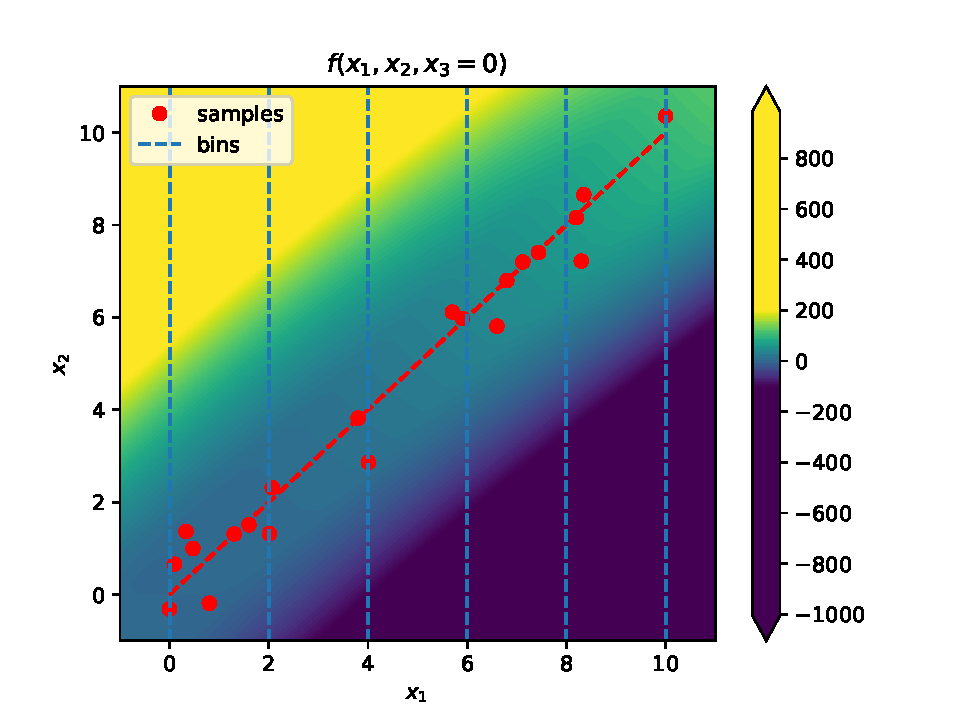
\includegraphics[width=.45\textwidth]{./../ACML-presentation/figures/bin_splitting_5_bins.pdf}
      \end{tabular} &
      \begin{tabular}{l}
        \parbox{0.49\linewidth}{Consider the following case; (a)
        we have limited samples (b) high variance in some features and (c) the black-box
        function changes abruptply outside of the data manifold. For example, \(
        f(x_1, x_2, x_3) = x_1x_2 + x_1x_3 \: \textcolor{red}{ \pm \: g(x)}\),
        with \(x_1 \in [0,10]\), \(x_2=x_1 + \epsilon\) and \(x_3 \sim
        \mathcal{N}(0, \sigma^2)\). The term \(x_1x_3\) makes estimations from
        limited samples (narrow bins) noisy, see Figure~\ref{fig:acc-1}.
        If we use larger bins (more \(\frac{\text{points}} { \text{bin}} \)),
        DALE leads to a good estimation whereas ALE fails due to OOD samples.}
      \end{tabular}
    \end{tabular}

    \begin{figure}
      \centering
      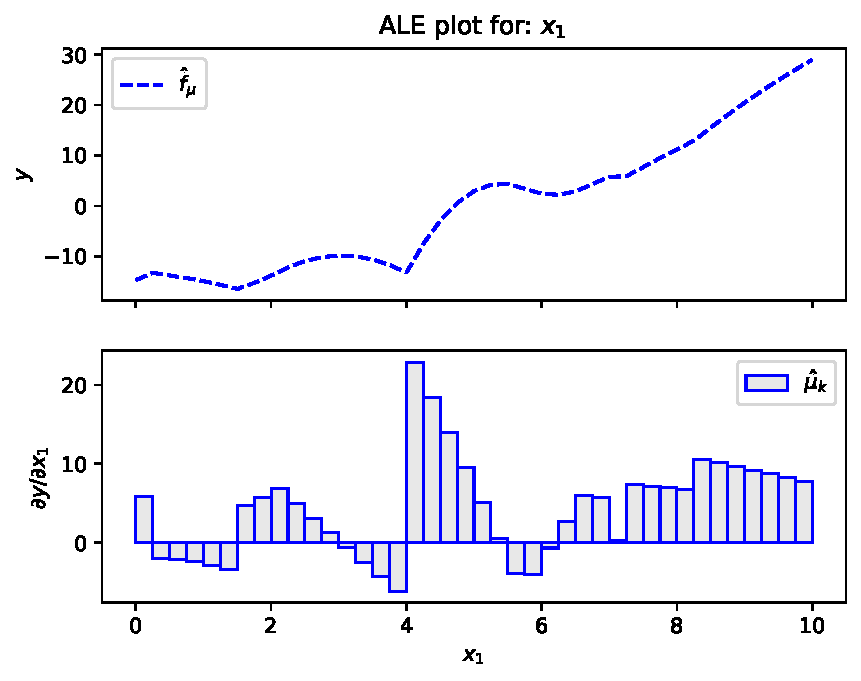
\includegraphics[width=0.49\textwidth]{./../ACML-presentation/figures/dale_40_bins.pdf}
      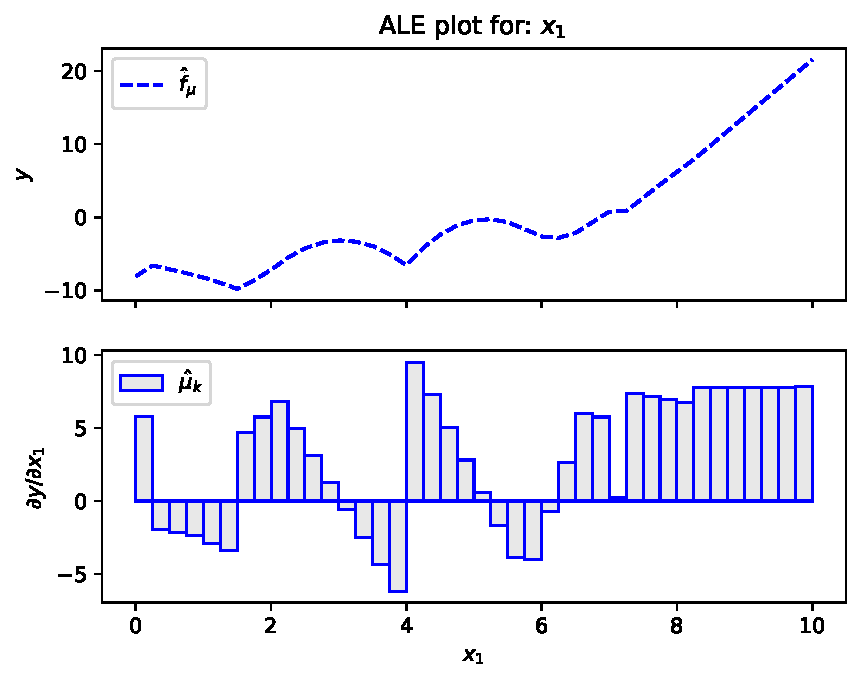
\includegraphics[width=0.49\textwidth]{./../ACML-presentation/figures/ale_40_bins.pdf}
      \caption{Narrow bins (\(K=40\)) \(\Rightarrow\) limited
        \(\frac{\text{samples}}{\text{bin}}\) \(\Rightarrow\) both plots are noisy }
      \label{fig:acc-1}
    \end{figure}

    \begin{figure} \centering
      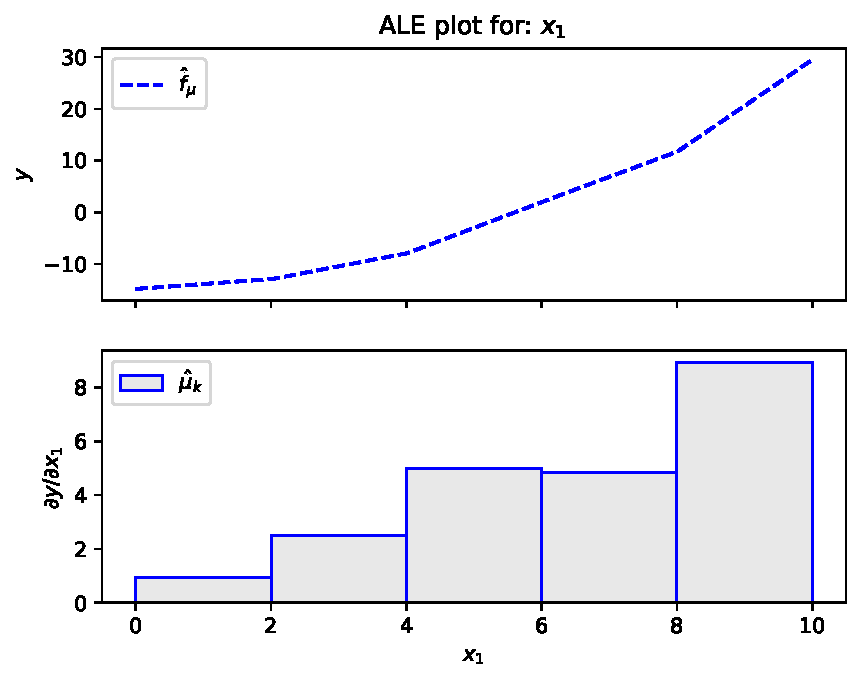
\includegraphics[width=0.49\textwidth]{./../ACML-presentation/figures/dale_5_bins.pdf}
      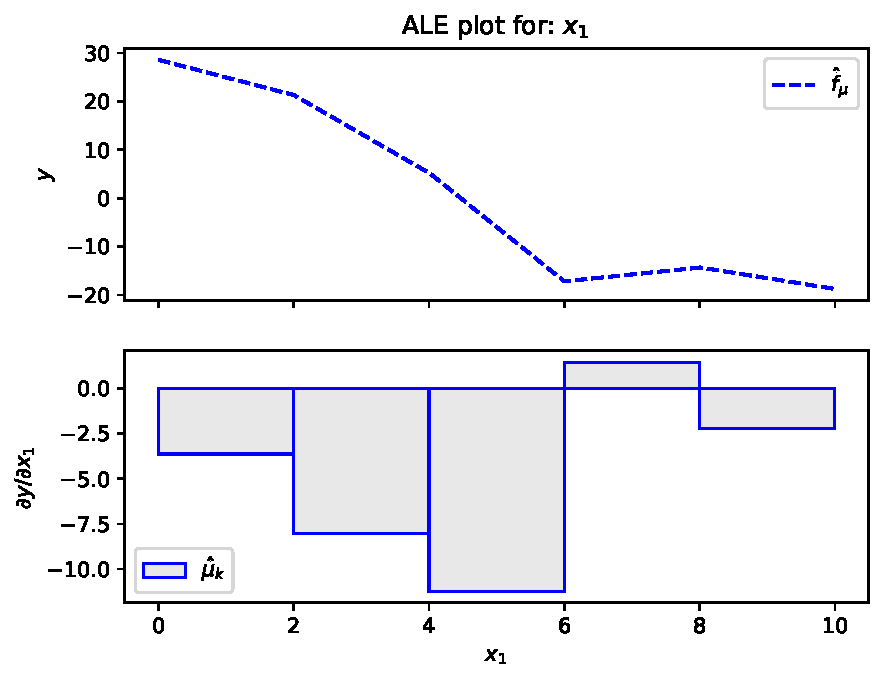
\includegraphics[width=0.49\textwidth]{./../ACML-presentation/figures/ale_5_bins.pdf}
      \caption{Wide bins (\(K=5\)) \(\Rightarrow\) many
        \(\frac{\text{samples}}{\text{bin}}\) \(\Rightarrow\) DALE is
        accurate, ALE is affected by OOD}
    \end{figure}
  \end{block}

  % DALE EFFICIENCY
  \begin{block}{DALE is fast}
    In a large and high dimensional dataset, ALE needs 10 mins, DALE some seconds!

    We test DALE vs ALE in two setups
    (Figure~\ref{fig:efficiency}). The light and heavy setup differ in
    the size of the dataset (\(N=10^2\) vs \(N=10^5\) instances) and
    the cost of evaluating \(f\) (light vs heavy). In both cases, DALE
    scales much better wrt dimensionality D.
    \begin{figure}[ht] \centering
      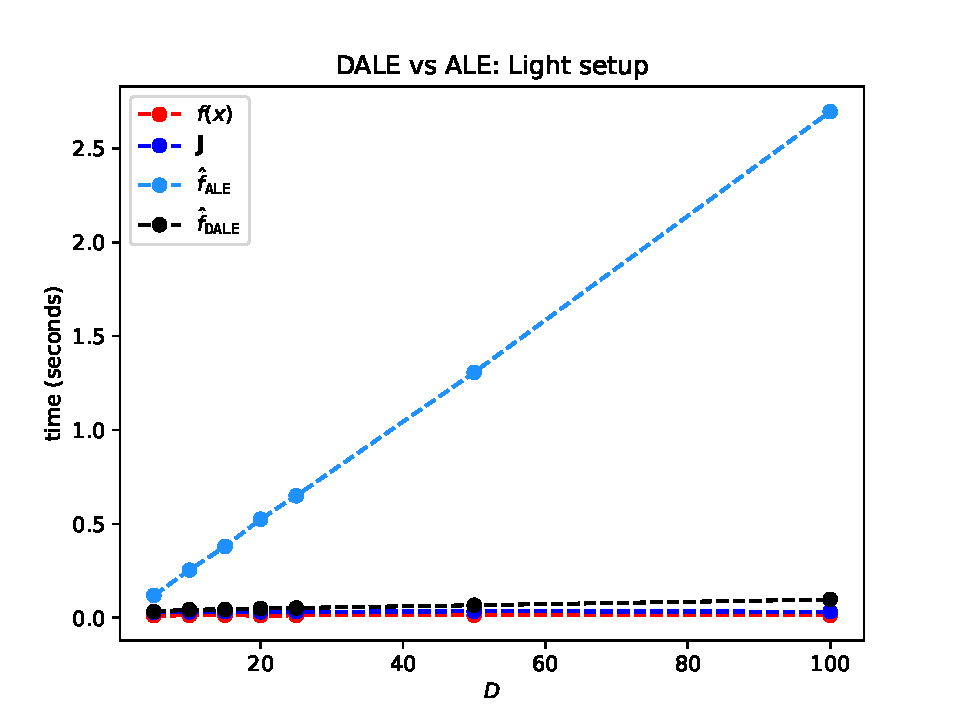
\includegraphics[width=0.49\textwidth]{./../ACML-paper/images/case-1-plot-1.pdf}
      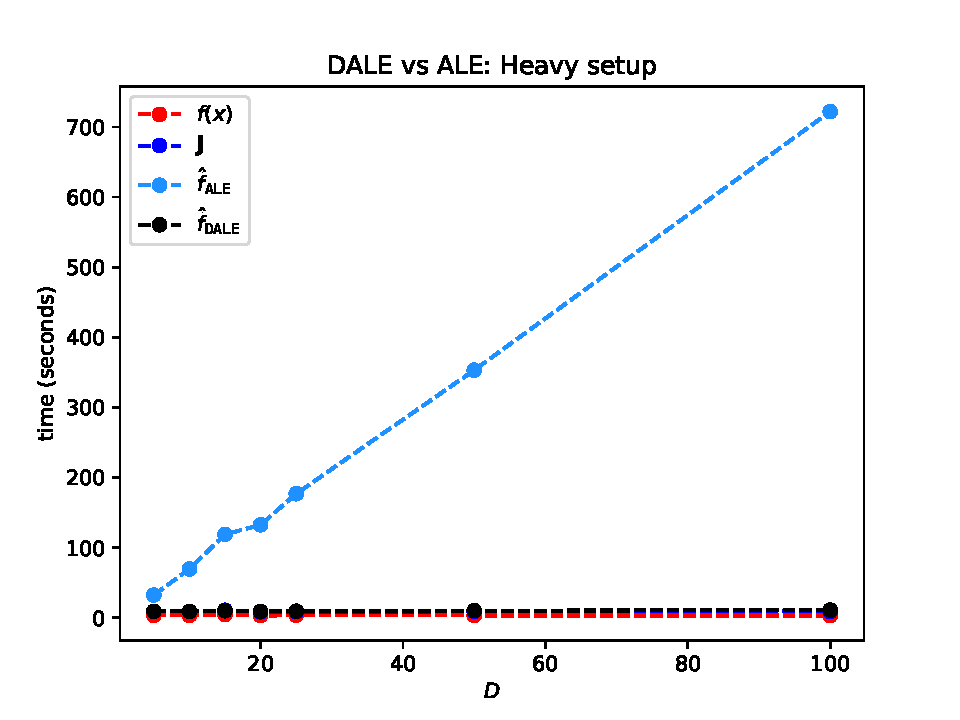
\includegraphics[width=0.49\textwidth]{./../ACML-paper/images/case-1-plot-2.pdf}
      \caption[Case-1-fig-1]{Light setup; small dataset
        \((N=10^2\) instances), light \(f\). Heavy setup; big dataset
        (\(N=10^5\) instances), heavy \(f\)}
      \label{fig:efficiency}
    \end{figure}
  \end{block}
\end{column} \separatorcolumn
\end{columns}

\begin{columns}[t]\separatorcolumn
    \begin{column}{1.3\colwidth}
      \large
      \begin{alertblock}{Conclusion} In case you work with a
        differentiable model, as in Deep Learning, use DALE to:
        \begin{itemize}
        \item compute the effect of all features efficiently
        \item test the FE plot for many different bin sizes \(K\), without computational cost
        \item ensure on-distribution estimation, irrespectively of the bin size
      \end{itemize}
    \end{alertblock}
	\end{column} \separatorcolumn
	\begin{column}{0.7\colwidth}
    \begin{block}{References}
      \printbibliography[heading=none]
      \begin{itemize}
      \item \large \href{givasile.github.io}{givasile.github.io}, \href{https://twitter.com/givasile1}{twitter.com/givasile1}
      \end{itemize}
      
	\end{block}
\end{column}
\separatorcolumn
\end{columns}


\end{frame}

\end{document}